We will evaluate the performance of the portfolio based on a mix of sharpe ratio and sortino ratio (achieved over a certain lookback period), somehow taking into account the diversification benefit of a portfolio allocation. We will also take into account how much a portfolio will be different from the previous one with a norm-1 penalty.
So our fitness function will look like:\\

$$
f_f = \alpha_1*sharpe(\mathbf{w}) + \alpha_2*sortino(\mathbf{w}) - \alpha_3*||\mathbf{w} - \mathbf{w_{old}}||
$$

Where $\alpha_1$, $\alpha_2$, and $\alpha_3$ are weights on which no optimization will be carried to limit the computaional burden. $\alpha_1$ and $\alpha_2$ will be the same, while $\alpha_3$ will be such that the influence on the optimal portfolio is relevant but still not that big to prevent the portfolio form evolving towards ones with better performance. In other wordsd, if an optimal portfolio is really different from the one traded the previous week, it must mean that the performance of the former must be really good to make us switch towards it incurring in relevant transaction costs.\\ 
We need to assign proper values for those three parameters in a way that it makes sense. We will give more relative weight to performance measures such as sharpe and sortino ratios and a bit less to the stability of the portfolio. To do this we take into account the order of magnitude of our scores. The sharpe ratio will be in absolute value normally in the range between 0 and 1.5 (we will not annualize the ratios as we care only about comparing performances, this way we will save some computations). The sortino ratio will be in the range between 0 and 3 in the most realistic cases.\\
For wat concerns the order of magnitude of the 1-norm we need to dig into some mathematics. We will generate the random weights for each portfolio manager as uniform values in the range $[0,1]$. The value of the norm-1 will be the sum of the absolute value of the difference of N uniform random variables. We will compute in the end the expected value of this norm-1. Let's set $\mathbf{X}, \mathbf{Y} \stackrel{i.i.d.}{\sim} \mathcal{U}(0,1)$.\\
\begin{equation} \label{first_step}
\mathbb{P}\left(\left\lVert\mathbf{X} - \mathbf{Y}\right\rVert < k\right) = \mathbb{P}\left(\mathbf{X} - k < \mathbf{Y} < \mathbf{X} + k\right)
\end{equation}  
We can easily visualize this simple problem on the $\mathbf{X}-\mathbf{Y}$ plane.\\

\begin{center}
	\centering
	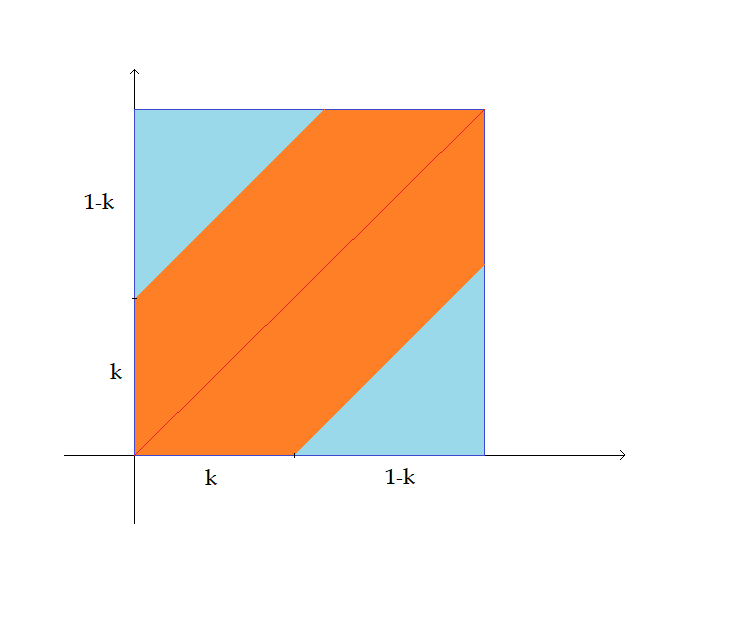
\includegraphics[width=0.6\textwidth]{Genetic_Algo/Prob_Square.png}
	\captionof{figure}{X-Y plane representation of the problem}
	\label{X_Y_plane}
\end{center}

The red area represents out probability. It is quite straightforward to notice that the area is equal to $1 - (1-k)^2 = 2k - k^2$. We can now extract the pdf of this particular random variable:

\begin{equation} \label{pdf}
f_{\left \lVert \mathbf{X} - \mathbf{Y}\right\rVert}(k) = \frac{dF_{\left \lVert \mathbf{X} - \mathbf{Y}\right\rVert}}{dx} = 2 - 2k \mathbf{1}_{[0,1]}(k)
\end{equation}

Now we can compute the expected value with the normal laws of probability:

\begin{equation} \label{expected_value}
\mathbb{E}\left[\left \lVert \mathbf{X} - \mathbf{Y}\right\rVert\right]  = \int_0^1 kf_{\left \lVert \mathbf{X} - \mathbf{Y}\right\rVert}(k)dk = k^2 - \frac{2}{3}k^3 \Big| _0^1 = \frac{1}{3}
\end{equation}

So the expected value of the norm difference for any portfolio will be $\frac{N}{3}$, where N is the number of assets in the portfolio (each week these are roughly 50-60). This means that this third element will be much greater in magnitude than the performance measures. We will need to set a value for $\alpha_3$ about 20 times smaller than $\alpha_1$ and $\alpha_2$. Since the scores will be relative to each other we don't care about the scale of the values, but only about the relative sizes. We therefore decide to set $\alpha_1 = \alpha_2 = 0.5$ and subsequently $\alpha_3 = 0.025$. 


